%%%%%%%%%%%%%%%%%%%%%%%%%%%%% Define Article %%%%%%%%%%%%%%%%%%%%%%%%%%%%%%%%%%
\documentclass{article}
%%%%%%%%%%%%%%%%%%%%%%%%%%%%%%%%%%%%%%%%%%%%%%%%%%%%%%%%%%%%%%%%%%%%%%%%%%%%%%%

%%%%%%%%%%%%%%%%%%%%%%%%%%%%% Using Packages %%%%%%%%%%%%%%%%%%%%%%%%%%%%%%%%%%
\usepackage{geometry}
\usepackage{graphicx}
\usepackage{amssymb}
\usepackage{amsmath}
\usepackage{amsthm}
\usepackage{empheq}
\usepackage{mdframed}
\usepackage{booktabs}
\usepackage{lipsum}
\usepackage{graphicx}
\usepackage{color}
\usepackage{psfrag}
\usepackage{pgfplots}
\usepackage{bm}
%%%%%%%%%%%%%%%%%%%%%%%%%%%%%%%%%%%%%%%%%%%%%%%%%%%%%%%%%%%%%%%%%%%%%%%%%%%%%%%

% Other Settings

%%%%%%%%%%%%%%%%%%%%%%%%%% Page Setting %%%%%%%%%%%%%%%%%%%%%%%%%%%%%%%%%%%%%%%
\geometry{a4paper}

%%%%%%%%%%%%%%%%%%%%%%%%%% Define some useful colors %%%%%%%%%%%%%%%%%%%%%%%%%%
\definecolor{ocre}{RGB}{243,102,25}
\definecolor{mygray}{RGB}{243,243,244}
\definecolor{deepGreen}{RGB}{26,111,0}
\definecolor{shallowGreen}{RGB}{235,255,255}
\definecolor{deepBlue}{RGB}{61,124,222}
\definecolor{shallowBlue}{RGB}{235,249,255}
%%%%%%%%%%%%%%%%%%%%%%%%%%%%%%%%%%%%%%%%%%%%%%%%%%%%%%%%%%%%%%%%%%%%%%%%%%%%%%%

%%%%%%%%%%%%%%%%%%%%%%%%%% Define an orangebox command %%%%%%%%%%%%%%%%%%%%%%%%
\newcommand\orangebox[1]{\fcolorbox{ocre}{mygray}{\hspace{1em}#1\hspace{1em}}}
%%%%%%%%%%%%%%%%%%%%%%%%%%%%%%%%%%%%%%%%%%%%%%%%%%%%%%%%%%%%%%%%%%%%%%%%%%%%%%%

%%%%%%%%%%%%%%%%%%%%%%%%%%%% English Environments %%%%%%%%%%%%%%%%%%%%%%%%%%%%%
\newtheoremstyle{mytheoremstyle}{3pt}{3pt}{\normalfont}{0cm}{\rmfamily\bfseries}{}{1em}{{\color{black}\thmname{#1}~\thmnumber{#2}}\thmnote{\,--\,#3}}
\newtheoremstyle{myproblemstyle}{3pt}{3pt}{\normalfont}{0cm}{\rmfamily\bfseries}{}{1em}{{\color{black}\thmname{#1}~\thmnumber{#2}}\thmnote{\,--\,#3}}
\theoremstyle{mytheoremstyle}
\newmdtheoremenv[linewidth=1pt,backgroundcolor=shallowGreen,linecolor=deepGreen,leftmargin=0pt,innerleftmargin=20pt,innerrightmargin=20pt,]{theorem}{Theorem}[section]
\theoremstyle{mytheoremstyle}
\newmdtheoremenv[linewidth=1pt,backgroundcolor=shallowBlue,linecolor=deepBlue,leftmargin=0pt,innerleftmargin=20pt,innerrightmargin=20pt,]{definition}{Definition}[section]
\theoremstyle{myproblemstyle}
\newmdtheoremenv[linecolor=black,leftmargin=0pt,innerleftmargin=10pt,innerrightmargin=10pt,]{problem}{Problem}[section]
%%%%%%%%%%%%%%%%%%%%%%%%%%%%%%%%%%%%%%%%%%%%%%%%%%%%%%%%%%%%%%%%%%%%%%%%%%%%%%%

%%%%%%%%%%%%%%%%%%%%%%%%%%%%%%% Plotting Settings %%%%%%%%%%%%%%%%%%%%%%%%%%%%%
\usepgfplotslibrary{colorbrewer}
\pgfplotsset{width=8cm,compat=1.9}
%%%%%%%%%%%%%%%%%%%%%%%%%%%%%%%%%%%%%%%%%%%%%%%%%%%%%%%%%%%%%%%%%%%%%%%%%%%%%%%

%%%%%%%%%%%%%%%%%%%%%%%%%%%%%%% Title & Author %%%%%%%%%%%%%%%%%%%%%%%%%%%%%%%%
\title{Maximum and Minimum}
\author{Patrick Chen}
\date{Oct 3, 2024}
%%%%%%%%%%%%%%%%%%%%%%%%%%%%%%%%%%%%%%%%%%%%%%%%%%%%%%%%%%%%%%%%%%%%%%%%%%%%%%%

\begin{document}
    \maketitle
    A absolute maximum is the maximum value that a function can produce. The
    absolute minimum is the minimum value that a function can produce. A local
    maximum is a point where any direction in the input space will produce a
    lesser value and likewise for local minimum. A point can be both a absolute
    maximum and local maximum. If function is undefined to the left or right of
    a point (blue graph at $(0,1)$), then it cannot be an local max or min.

    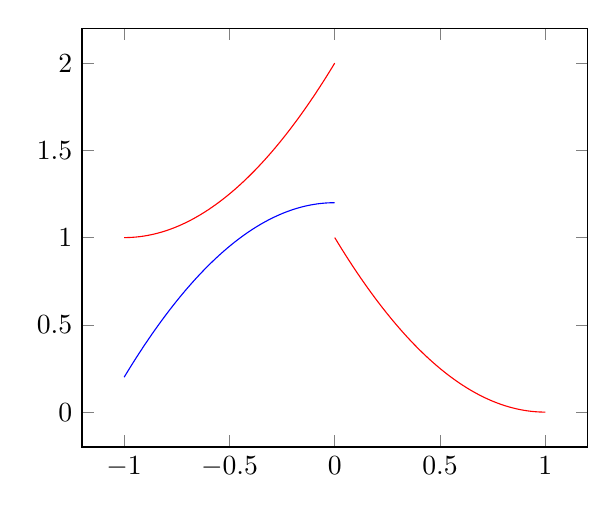
\begin{tikzpicture}
         \begin{axis}
             \addplot [
                domain=-1:0,
                samples=70,
                color=blue,
                ]
                {-x^2+1.2};
             \addplot [
                domain=0:1,
                samples=70,
                color=red,
                ]
                {(x-1)^2};
             \addplot [
                domain=-1:0,
                samples=70,
                color=red,
                ]
                {(x+1)^2+1};
         \end{axis}
    \end{tikzpicture}

    If a function has a "max", but it is on a open interval and thus not part of
    the graph, then it is not considered a max.

    \subsection*{Extreme Value Theorem}
    If f is continuous on a closed interval [a,b], the then f attains an
    absolute maximum value f(c) and an absolute minimum value f(d) at some
    numbers c and d in [a,b].

    \subsection*{Fermat's Theorem}
    If $f$ has a local maximum or minimum at $c$, and $f'(c)$ exists, then
    $f'(c)=0$. Note that if the derivative is zero, that does not necessary
    mean that a local extreme exists. Local extreme values can also happen when
    $f(c)\ne 0$. When the derivative $f'(c)$ is zero or does not exists, then
    $c$ is considered a critical number.

    \subsection*{Finding Maximum and Minimum}
    The absolute maximum and minimum of a continuous function on the closed
    interval $[a,b]$ can be found by following these steps:

    \begin{enumerate}
        \item Find the values of f at the critical numbers of f in (a,b)
        \item Find the values of f at the endpoints of the interval
        \item The largest of the values from steps 1 and 2 is the absolute
            maximum and the least of the values is the absolute minimum on the
            interval [a,b]
    \end{enumerate}

    \subsection*{Example}
    \begin{align*}
        f(x)  &= 2\cos x + \sin 2x \\
        f'(x) &= -2\sin x + 2\cos2x \\
        0 &= -\sin x + \cos 2x \\
        0 &= -\sin x + \cos^2 x - \sin^2 x \\
        0 &= -\sin x + 1 - \sin^2 x - \sin^2 x \\
        0 &= -2\sin^2 x -\sin x + 1 \\
        \sin x &= \frac{-1 \pm 3}{4} \\
        \sin x &= -1, \frac{1}{2} \\
        x &= \frac{3\pi}{2}, \frac{\pi}{6}, \frac{5\pi}{6}
    \end{align*}

\end{document}
